% ===============================================================
% TEMPLATE DE APRESENTAÇÃO (BEAMER) - TCC1 - SENAC SANTO AMARO
% ===============================================================
% Apresentação da PROPOSTA de Trabalho de Conclusão de Curso (TCC1)
%
% >>> DURAÇÃO DA APRESENTAÇÃO: 20 MINUTOS <<<
%
% A apresentação DEVE seguir a mesma estrutura do documento escrito
% (arquivo tcc.tex), na ordem:
%   1. Introdução (Contexto, Justificativa, Objetivos)
%   2. Referencial Bibliográfico (Metodologia da pesquisa,
%      Referencial, Trabalhos relacionados)
%   3. Desenvolvimento (Solução proposta, Cronograma)
%
% LOGO: a logo do SENAC aparece GRANDE no primeiro slide (capa) e
% PEQUENA no canto superior direito dos demais slides.
% Coloque o arquivo da logo em:  assets/logo-senac.png
% (Se o arquivo não existir, um marcador de texto é exibido no lugar
%  para que a apresentação compile mesmo assim.)
%
% COMO COMPILAR:
%   pdflatex apresentacao_tcc1.tex
%   pdflatex apresentacao_tcc1.tex   (2x para fixar índice/numeração)
% ===============================================================

\documentclass[
    aspectratio=169,   % proporção 16:9 (use 43 para 4:3)
    12pt,
    brazil
]{beamer}

% ---------------------------------------------------------------
% PACOTES
% ---------------------------------------------------------------
\usepackage[T1]{fontenc}
\usepackage[utf8]{inputenc}
\usepackage[brazil]{babel}
\usepackage{graphicx}
\usepackage{booktabs}
\usepackage{tikz}
\usepackage{pgfgantt}
\usepackage{appendixnumberbeamer}
\usepackage{lmodern}                % Fonte Latin Modern
\usepackage{color}                  % Controle de cores
\usepackage{microtype}              % Melhorias de justificação
\usepackage{float}                  % Para posicionamento de figuras
\usepackage[brazilian,hyperpageref]{backref}  % Páginas com citações
\usepackage[alf]{abntex2cite}


\hypersetup{
    pdfcreator={LaTeX with abnTeX2},
    pdfkeywords={tcc}{senac}{santo amaro}{trabalho de conclusão},
    colorlinks=true,        % false: links em caixas; true: links coloridos
    linkcolor=.,         % cor dos links internos
    citecolor=blue,         % cor dos links para bibliografia
    filecolor=magenta,      % cor dos links para arquivos
    urlcolor=blue,
    bookmarksdepth=4
}


% ---------------------------------------------------------------
% TEMA E CORES
% ---------------------------------------------------------------
\usetheme{default}
\useinnertheme{circles}
\setbeamertemplate{navigation symbols}{}   % remove ícones de navegação

% Cores institucionais (ajuste se o curso definir outras)
\definecolor{senacblue}{RGB}{0,51,102}
\definecolor{senacorange}{RGB}{243,146,0}

\setbeamercolor{structure}{fg=senacblue}
\setbeamercolor{frametitle}{fg=white,bg=senacblue}
\setbeamercolor{title}{fg=senacblue}
\setbeamercolor{section in toc}{fg=senacblue}
\setbeamercolor{itemize item}{fg=senacorange}
\setbeamercolor{itemize subitem}{fg=senacorange}
\setbeamerfont{frametitle}{series=\bfseries}
\setbeamertemplate{frametitle}[default][left]
\setbeamertemplate{caption}[numbered]
\setbeamerfont{caption name}{series=\bfseries}

% Rodapé simples: autor | título curto | número do slide
\setbeamertemplate{footline}{%
  \leavevmode%
  \hbox{%
    \begin{beamercolorbox}[wd=.34\paperwidth,ht=2.4ex,dp=1ex,leftskip=1em]{author in head/foot}%
      \usebeamerfont{author in head/foot}\insertshortauthor
    \end{beamercolorbox}%
    \begin{beamercolorbox}[wd=.5\paperwidth,ht=2.4ex,dp=1ex,center]{title in head/foot}%
      \usebeamerfont{title in head/foot}\insertshorttitle
    \end{beamercolorbox}%
    \begin{beamercolorbox}[wd=.16\paperwidth,ht=2.4ex,dp=1ex,rightskip=1em]{title in head/foot}%
      \usebeamerfont{title in head/foot}\hfill\insertframenumber/\inserttotalframenumber
    \end{beamercolorbox}%
  }\vskip0pt%
}
\setbeamercolor{author in head/foot}{bg=senacblue,fg=white}
\setbeamercolor{title in head/foot}{bg=senacblue!85,fg=white}

% ---------------------------------------------------------------
% LOGO DO SENAC (grande na capa, pequena no canto dos demais slides)
% ---------------------------------------------------------------
% Macro para a logo GRANDE (capa).
\newcommand{\logosenacgrande}{%
  \IfFileExists{Images/logo-senac.png}{%
    
\includegraphics[height=2.6cm]{Images/logo-senac.png}%
  }{%
    \begin{tikzpicture}
      \node[draw=senacblue,line width=1pt,rounded corners,
            minimum width=4.5cm,minimum height=2.4cm,align=center,
            fill=senacblue!5]
        {\bfseries\color{senacblue}\Large SENAC\\[2pt]
         \normalsize Santo Amaro\\[6pt]
         \scriptsize\itshape (coloque assets/logo-senac.png)};
    \end{tikzpicture}%
  }%
}

% Macro para a logo PEQUENA (canto superior direito).
\newcommand{\logosenacpequena}{%
  \IfFileExists{Images/logo-senac.png}{%
    
\includegraphics[height=0.5cm]{Images/logo-senac.png}%
  }{%
    \fbox{\scriptsize\bfseries\color{senacblue}SENAC}%
  }%
}

% Coloca a logo pequena no canto superior direito dos slides que têm
% título (sobre a barra azul, dentro de um pequeno "chip" branco para
% que a logo preta fique visível). Os frames "plain" (capa e
% encerramento) não têm frametitle, logo não recebem a logo pequena
% --- exatamente como desejado.
\newcommand{\minhaspaginas}{}

\setbeamertemplate{frametitle}{
  \nointerlineskip
  \begin{beamercolorbox}[wd=\paperwidth, ht=0.55cm, dp=0.2cm, leftskip=0.3cm, rightskip=1.5cm]{frametitle}
    \usebeamerfont{frametitle}\insertframetitle 
    \hfill \usebeamerfont{title in head/foot}\minhaspaginas
  \end{beamercolorbox}
}

\addtobeamertemplate{frametitle}{}{%
  \begin{tikzpicture}[remember picture,overlay]
    \node[anchor=north east,fill=white,rounded corners=2pt,inner sep=3pt]
      at ([xshift=-6pt,yshift=-5pt]current page.north east) {\logosenacpequena};
  \end{tikzpicture}%
}

% ---------------------------------------------------------------
% DADOS DA APRESENTAÇÃO (preencha)
% ---------------------------------------------------------------
\title[Análise Estática Generativa com LLMs]{Análise Estática Generativa com LLMs: Otimizando a Detecção de Vulnerabilidades no SemGrep via Abordagem Multi-Agente}
\subtitle{TCC1}
\author[Caio Xavier da Silva]{Caio Xavier da Silva}
\institute[SENAC Santo Amaro]{%
  SENAC --- Unidade Santo Amaro\\
Bacharelado em Ciência da Computação}
\date{
  Orientador: Leonardo Massayuki Takuno \\
  \footnotesize Coorientador: Thyago Conchado Quintas \\
  São Paulo, 2025}

% ===============================================================
\begin{document}

% ---------------------------------------------------------------
% SLIDE 1 - CAPA (logo GRANDE)  -- ~0:30
% ---------------------------------------------------------------
{
\setbeamertemplate{footline}{}   % capa sem rodapé
\begin{frame}[plain]
  \centering
  \vspace{0.3cm}
  \logosenacgrande\par
  \vspace{0.05cm}
  {\usebeamerfont{title}\usebeamercolor[fg]{title}\bfseries\inserttitle\par}
  \vspace{0.3cm}
  {\insertauthor\par}
  \vspace{0.15cm}
  {\footnotesize\insertinstitute\par}
  \vspace{0.25cm}
  {\footnotesize\insertdate\par}
\end{frame}
}

% ---------------------------------------------------------------
% SLIDE 2 - AGENDA / ROTEIRO  -- ~0:30
% ---------------------------------------------------------------
\begin{frame}{Roteiro da apresentação}
  \tableofcontents
\end{frame}

% ===============================================================
% A ORDEM ABAIXO SEGUE EXATAMENTE O DOCUMENTO ESCRITO (tcc.tex)
% Sugestão de tempo total: 20 minutos
%   - Introdução .................. ~5 min
%   - Referencial Bibliográfico ... ~5 min
%   - Desenvolvimento ............. ~7 min
%   - Encerramento ................ ~3 min
% Regra prática: ~1 a 1,5 min por slide => ~14 a 18 slides de conteúdo.
% Reserve ~2 a 3 min para perguntas da banca, dentro dos 20 min.
% ===============================================================

% ---------------------------------------------------------------
\section{Introdução}
% ---------------------------------------------------------------

\renewcommand{\minhaspaginas}{\small 8 - 9}
\begin{frame}{Introdução}
  \begin{itemize}
    \item Análise estática e sua utilização.
      \tab {\footnotesize \cite{hou2025generation, jiang2025factaligned}}
    \item \textbf{Limitações da análise estática tradicional}:
      \begin{itemize}
        \item Escalabilidade e Diversidade de \textit{Bugs};
          \tab {\footnotesize \cite{yang2025knighter}}
        \item Esforço Humano;
          \tab {\footnotesize \cite{hou2025generation}}
        \item Falta de Extensibilidade Multilinguagem;
          \tab {\footnotesize \cite{hou2025generation}}
        \item Falsos Positivos e Falsos Negativos.
          \tab {\footnotesize \cite{jiang2025factaligned}}
      \end{itemize}
  \end{itemize}
\end{frame}

\renewcommand{\minhaspaginas}{\small 9 - 11}
\begin{frame}{Contexto}
  \begin{itemize}
    \item LLMs na análise estática.
    \tab {\footnotesize \cite{tang2021grammar, yang2025knighter}}
    \item \textbf{Limitações desses modelos}:
    \tab {\footnotesize \cite{tunstall2022natural, hou2025generation}}
    \begin{itemize}
      \item Custos proibitivos (milhões de \textit{tokens});
      \item Restrições práticas (\textit{self-attention}).
    \end{itemize}
  \end{itemize}
\end{frame}

\renewcommand{\minhaspaginas}{\small 11}
\begin{frame}{Contexto}
  \begin{itemize}
    \item \textbf{Multi-Agentes}:
    \tab {\footnotesize \cite{russell2020artificial}}
    \begin{itemize}
      \item Processamento descentralizado e distribuído entre agentes;
      \item Cada agente assume um papel restrito e especializado;
      \item Reduzir sobrecarga de \textit{tokens};
      \item Maior precisão na geração do artefato final.
    \end{itemize}
    \item \textbf{Analisador estático ideal}:
    \tab {\footnotesize \cite{yang2025knighter}}
    \begin{itemize}
      \item Detectar uma diversidade de falhas;
      \item Eficientemente processar milhões de linhas de código.
    \end{itemize}
    \item Motivações (Figura \ref{fig:motivacoes}).
    \tab {\footnotesize \cite{yang2025knighter}}
  \end{itemize}
\end{frame}

\renewcommand{\minhaspaginas}{\small 10}
\begin{frame}{Contexto - Figura 1}
  \vspace{-0.85cm} \begin{figure}[h]
    \centering
    \caption{Motivação para \textit{checkers} feitos por llms.}
    \includegraphics[width=0.98\textwidth]{Images/problemas em larga escala-sideways.png} \\
    {\small Fonte: Adaptado pelo autor para melhor compreensão \cite{yang2025knighter}}
    \label{fig:motivacoes}
  \end{figure}
\end{frame}

\renewcommand{\minhaspaginas}{\small 12}
\begin{frame}{Justificativa}
  \begin{itemize}
    \item LLMs na análise estática.
    \tab {\footnotesize \cite{hou2025generation, yang2025knighter, li2026llmbased}}
    \item \textbf{Limites desse método}:
    \tab {\footnotesize \cite{hou2025generation, yang2025knighter, li2026llmbased}}
    \begin{itemize}
      \item Cobertura limitada;
      \item Falha em variações semânticas complexas;
      \item \textit{corner-cases}.
    \end{itemize}
  \item Análise estática via regras (SemGrep, Figura \ref{fig:exemplosemgrep}).
  \end{itemize}
\end{frame}

\renewcommand{\minhaspaginas}{\small 13}
\begin{frame}{Justificativa}
  \setbeamerfont{caption}{size=\scriptsize}
  \vspace{-0.85cm}\begin{figure}[h]
    \centering
    \caption{Exemplo de regra criada para detectar uma senha embutida no argumento da função em Python.}
    \vspace{-0.25cm}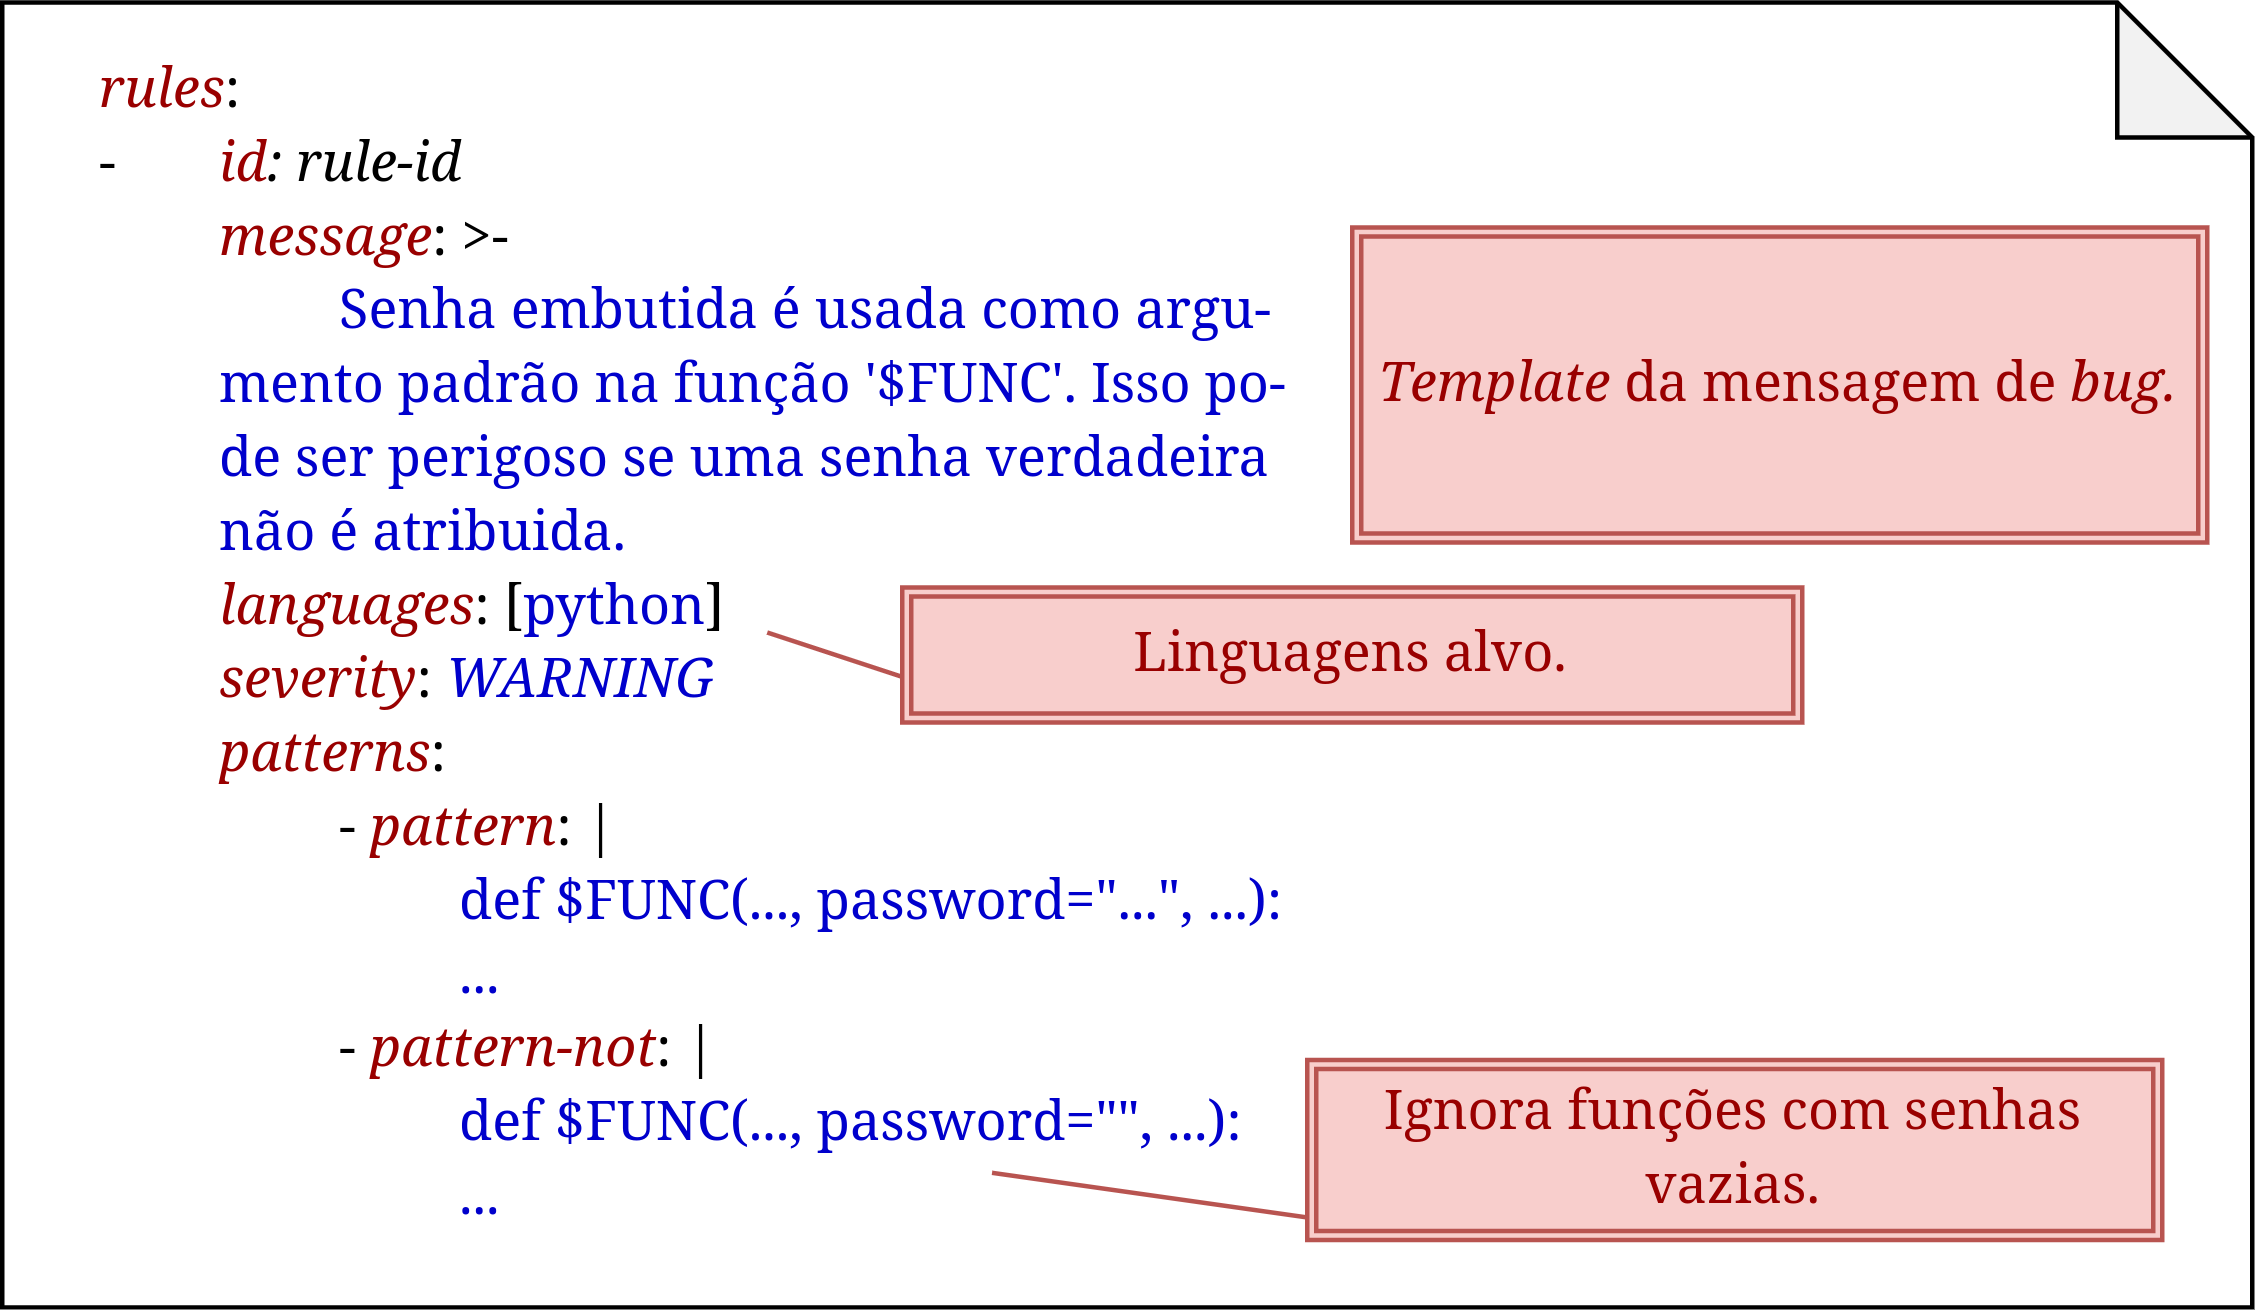
\includegraphics[width=0.82\textwidth]{Images/Semgrep.png} \\
    {\scriptsize Fonte: Adaptado para português com finalidade de melhorar compreensão \cite{hou2025generation}}
    \label{fig:exemplosemgrep}
  \end{figure}
\end{frame}

\renewcommand{\minhaspaginas}{\small 12}
\begin{frame}{Justificativa}
  \begin{block}{Justificativa formal}
    Portanto, este trabalho justifica-se pela necessidade de preencher a atual lacuna de eficácia e escalabilidade na detecção de vulnerabilidades.
    O desenvolvimento de um \textit{framework} iterativo, focado na geração automatizada de regras para o motor do SemGrep, é motivado em mitigar a dependência de engenharia manual e contornar os altos custos da inferência direta por IAs.
    Ao propor um sistema especializado nas vulnerabilidades críticas (CWEs) da linguagem C, essa pesquisa visa demonstrar que é possível identificar padrões semânticos e \textit{corner-cases} com maior precisão e viabilidade técnica do que os analisadores estáticos tradicionais ou métodos generalistas baseados exclusivamente em LLMs.
  \end{block}
\end{frame}

\begin{frame}{Hipótese}
  \begin{block}{Hipótese formal}
    A hipótese desta pesquisa é a de que a geração automatizada de regras por meio de um \textit{framework} multi-agente baseado em LLMs, integrado ao motor do SemGrep, produzirá taxas de detecção (\textit{Recall} e \textit{F1-Score}) de vulnerabilidades (CWEs) em C estatisticamente superiores e com maior identificação de \textit{corner-cases} quando comparada aos conjuntos de regras predefinidas dos analisadores estáticos tradicionais (como por exemplo \textit{ruleset} tradicional do SemGrep).
  \end{block}
\end{frame}

\renewcommand{\minhaspaginas}{\small 13}
\begin{frame}{Objetivo}
  \begin{block}{Objetivo Geral}
    O objetivo geral deste trabalho é demonstrar que um \textit{framework} de síntese automatizada de regras, baseando-se em Modelos de Linguagem de Larga Escala e integrado à ferramenta SemGrep, apresenta precisão e \textit{recall} estatisticamente superiores às abordagens estáticas tradicionais na detecção de vulnerabilidades críticas em linguagem C.
    Busca-se demonstrar que este modelo supera abordagens estáticas tradicionais na identificação precisa de, no mínimo, cinco categorias de vulnerabilidades de software, em inglês \textit{Common Weakness Enumeration} (CWE).
  \end{block}
\end{frame}

\renewcommand{\minhaspaginas}{\small 13 - 14}
\begin{frame}{Objetivo}
  \begin{block}{Objetivos específicos}
    \begin{itemize}
      \item Determinar os limites de detecção semântica (\textit{corner-cases}) que podem ser superados pela abordagem gerativa de LLMs em relação aos conjuntos de regras predefinidas (\textit{ruleset}) estáticos.
      \item Estabelecer o ganho quantitativo de desempenho (\textit{Recall}, Precisão e F1-Score) de regras sintetizadas dinamicamente frente aos analisadores tradicionais do estado da arte.
      \item Determinar a viabilidade técnica e a escalabilidade de inferência da arquitetura proposta utilizando modelos de linguagem de menor escala (com contagem reduzida de parâmetros), visando garantir a viabilidade técnica da execução do \textit{framework} em infraestruturas locais com restrições de custo e \textit{hardware}.
    \end{itemize}
  \end{block}
\end{frame}

% ---------------------------------------------------------------
\section{Referencial Bibliográfico}
% ---------------------------------------------------------------

\renewcommand{\minhaspaginas}{\small 15}
\begin{frame}{Metodologia da pesquisa bibliográfica}
  \begin{itemize}
    \item \textbf{Motor de pesquisa}: Google Acadêmico.
    \item \textbf{Bases consultadas}: 
      \begin{itemize}
        \item IEEE Xplore;
        \item arXiv;
        \item ACM Digital Library.
      \end{itemize}
    \item \textbf{Palavras-chave}: Figura \ref{fig:keywords}.
  \end{itemize}
\end{frame}

\begin{frame}{Metodologia da pesquisa bibliográfica}
  \vspace{-0.85cm} \begin{figure}[h]
    \centering
    \caption{\textit{Query} utilizada durante a pesquisa de materiais.}
    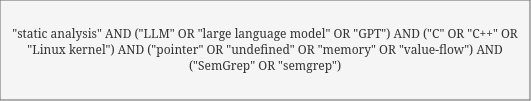
\includegraphics[width=1\textwidth]{Images/Query.png} \\
    {\small Fonte: Elaborado pelo autor (2026)}
    \label{fig:keywords}
  \end{figure}
\end{frame}

\renewcommand{\minhaspaginas}{\small 15 - 16}
\begin{frame}{Metodologia da pesquisa bibliográfica}
  \begin{block}{Critérios de Inclusão}
    \begin{enumerate}
      \item Trabalhos publicados entre 2021 e 2026;
      \item Disponibilidade nos idiomas inglês ou português;
      \item Relação direta com o tema.
    \end{enumerate}
  \end{block}
  \begin{block}{Critérios de Exclusão}
    \begin{enumerate}
      \item Trabalhos publicados antes de 2021; \\
        \hspace{0.2cm} {\small Exceção de referências clássicas/seminais.}
      \item Artigos sem alinhamento direto com análise estática \\
        ou geração de regras de código;
      \item Duplicidade de publicações.
    \end{enumerate}
  \end{block}
\end{frame}

\renewcommand{\minhaspaginas}{\small 16}
\begin{frame}{Metodologia da pesquisa bibliográfica}
  \begin{enumerate}
    \item \textbf{Primeira fase (triagem)}: 
      \begin{itemize}
        \item \textit{Query} retornou cerca de 4770 resultados.
        \item Selecionados 47 potencialmente relevantes.
      \end{itemize}
    \item \textbf{Segunda fase (afunilamento)}:
      \begin{itemize}
        \item Leitura de introdução e escopo.
        \item Classificação de 0 a 10 de acordo com os objetivos deste trabalho. \\
        \hspace{0.2cm} {\small Avaliação feita a partir de seu resumo, palavras-chave, tecnologias aplicadas}.
      \item Totalizando em 15 trabalhos conteporâneos (6 relevantes e 9 suporte).
      \item Adicionando 5 trabalhos seminais anteriores a 2021.
      \end{itemize}
  \end{enumerate}
\end{frame}

\begin{frame}{Metodologia da pesquisa bibliográfica}
  \setbeamerfont{caption}{size=\scriptsize}
  \vspace{-0.98cm}\begin{figure}[h]
    \centering
    \caption{Funil de pesquisa.}
    \vspace{-0.15cm}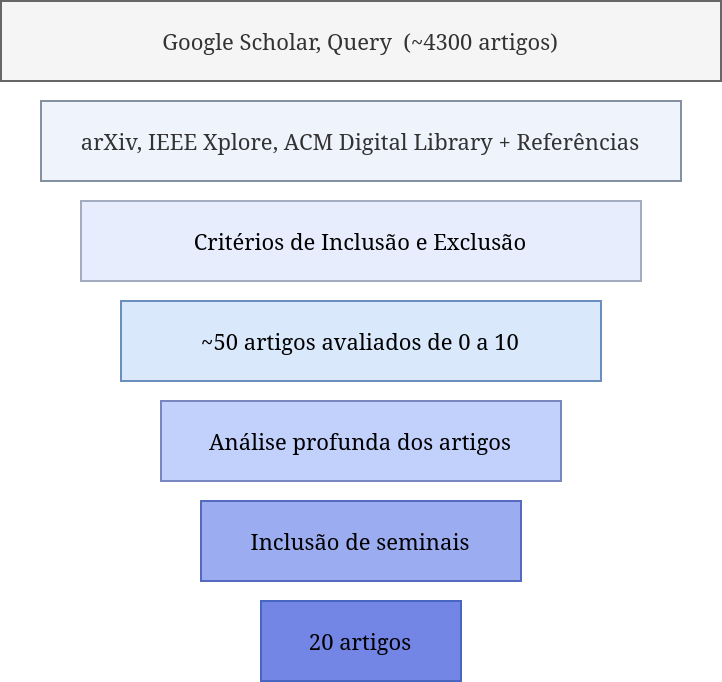
\includegraphics[width=0.53\textwidth]{Images/Funil.png} \\
    \vspace{-0.18cm}{\scriptsize Fonte: Elaborado pelo autor (2026)}
    \label{fig:funil}
  \end{figure}
\end{frame}

\renewcommand{\minhaspaginas}{\small 21 - 23}
\begin{frame}{Referencial teórico e técnico}
  \begin{block}{Análise Estática Baseada em Regras}
    \begin{itemize}
      \item Ferramentas relevantes: SemGrep e CodeQL.
        {\small \cite{jiang2025factaligned, hou2025generation}}
      \item \textbf{SemGrep}:
        \begin{itemize}
          \item Suporta estruturas complexas e verificações básicas de fluxo de dados.
          \item Gramática em YAML mimetiza a linguagem alvo.
          \item Curva de aprendizado é menor que CodeQL.
          \item Converte o código em uma árvore de sintaxe abstrata universal (UAST).
          \item Exemplo (Figura \ref{fig:semgrep}).
        \end{itemize}
    \end{itemize}
  \end{block}
\end{frame}

\begin{frame}{SemGrep}
  \vspace{-0.85cm} \begin{figure}[h]
    \centering
    \caption{Exemplo de regra simplificada para a detecção de falhas OSCI em Java.}
    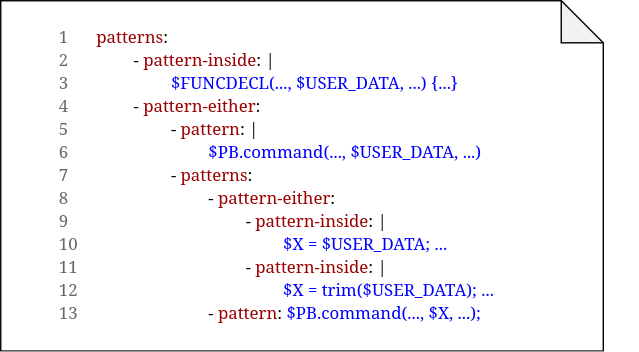
\includegraphics[width=0.85\textwidth]{Images/Semgrep-java.png} \\
    {\small Fonte: Adaptado de \cite{jiang2025factaligned}}
    \label{fig:semgrep}
  \end{figure}
\end{frame}

\begin{frame}{SemGrep}
  \textbf{SemGrep utiliza dois recursos fundamentais}:
  \begin{enumerate}
    \item \textbf{Metavariáveis}, auxiliando no fluxo de dados.
    \item \textbf{Curinga} (...), permitindo omitir detalhes não relevantes.
  \end{enumerate}
  \textbf{Predicados}:
  \begin{itemize}
    \item \textbf{\textit{patterns}}, representando \textit{AND} (E).
    \item \textbf{\textit{pattern-inside}}, define o contexto.
    \item \textbf{\textit{pattern-either}}, representa \textit{OR} (OU).
    \item \textbf{\textit{pattern-not}}, representa \textit{NOT} (NÃO).
  \end{itemize}
\end{frame}

\renewcommand{\minhaspaginas}{\small 23 - 24}
\begin{frame}{Referencial teórico e técnico}
  \begin{block}{Vulnerabilidades de Linguagem}
    \begin{itemize}
      \item Vulnerabilidade é um conjunto de condições que permite um invasor (atacante) viole uma política de segurança explícita ou implícita.
      {\small \cite{seacord2013secure}}
    \item \textbf{\textit{Common Weakness Enumeration}} é um dicionário formal desenvolvida pela comunidade que categoriza fraquezas comuns de \textit{software} e \textit{hardware}.
    \item \textbf{Fraquezas (\textit{Weakness})} é definido como uma condição que um componente de \textit{software, firmware, hardware} ou serviço pode contribuir para a introdução de uma vulnerabilidade.
      {\small \cite{mitrecwe}}
    \end{itemize}
  \end{block}
\end{frame}

\begin{frame}{Vulnerabilidades de Linguagem}
  \begin{block}{CWEs selecionadas}
    \begin{itemize}
      \item \textbf{CWE-401}: \textit{Missing Release of Memory after Effective Lifetime}; 
      \item \textbf{CWE-415}: \textit{Double Free}; 
      \item \textbf{CWE-416}: \textit{Use After Free}; 
      \item \textbf{CWE-457}: \textit{Use of Uninitialized Variable};
      \item \textbf{CWE-476}: \textit{Null Pointer Dereference}.
    \end{itemize}
  \end{block}
\end{frame}

\renewcommand{\minhaspaginas}{\small 36 - 38}
\begin{frame}{Trabalhos relacionados}
  \begin{block}{\textit{KNighter: Transforming Static Analysis with LLM-Synthesized Checkers} \cite{yang2025knighter}}
    \begin{itemize}
      \item  Publicado em SOSP 25 \textit{(ACM SIGOPS 31st Symposium on Operating Systems Principles)}, em Seul, República da Coreia.
      \item KNighter foi o primeiro sistema de geração de analisadores estáticos totalmente automatizado.
    \tab {\footnotesize \cite{yang2025knighter}}
      \item Motivado pelas limitações da análise estática tradicional.
      \item Propõe um \textit{framework} voltado à extração de \textit{commits}.
      \item \textit{Overview} do trabalho (Figura \ref{fig:knighter}).
    \end{itemize}
  \end{block}
\end{frame}

\renewcommand{\minhaspaginas}{\small 36 - 38}
\begin{frame}{KNighter}
  \begin{itemize}
    \item \textbf{Motor principal}: \textit{Clang Static Analyser} (CSA).
    \item Como \textit{commit} de entrada, KNighter retorna como saída um \textit{checker} para \textit{Clang Static Analyser} (CSA).
    \tab {\footnotesize \cite{yang2025knighter}} \\
    {\small Sendo um verificador válido aquele que identifica o código pré \textit{commit} como \textit{bug} e o código corrigido como correto.}
    \item \textbf{KNighter possui duas fases}: (Figura \ref{fig:knighter})
      \begin{itemize}
        \item Sintetização de verificadores;
        \item Reparo para erros.
      \end{itemize}
    \item \textbf{Diferenças do presente trabalho}:
      \begin{itemize}
        \item CSA vs. SemGrep;
        \item Utiliza somente \textit{commits} para geração de regras.
      \end{itemize}
  \end{itemize}
\end{frame}

\renewcommand{\minhaspaginas}{\small 37}
\begin{frame}{KNighter}
  \vspace{-0.85cm} \begin{figure}[h]
    \centering
    \caption{\textit{Overview} do KNighter.}
    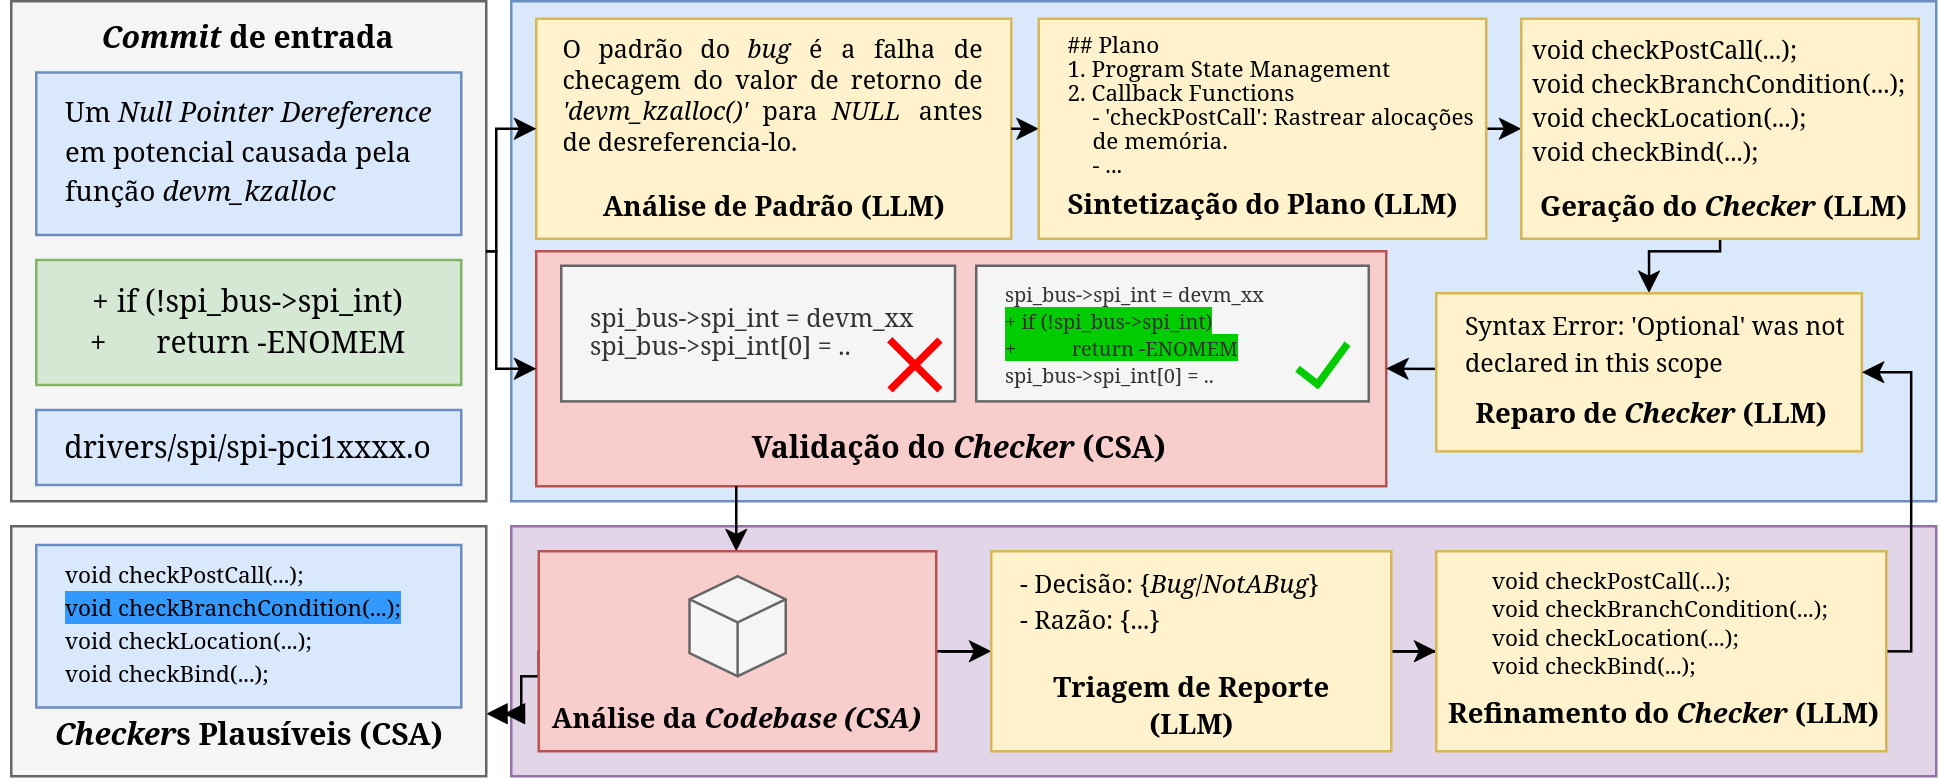
\includegraphics[width=1\textwidth]{Images/Overview-KNighter.png} \\
    {\small Fonte: Adaptado para o português para melhor compreensão \cite{yang2025knighter}}
    \label{fig:knighter}
  \end{figure}
\end{frame}

\renewcommand{\minhaspaginas}{\small 38 - 40}
\begin{frame}{Trabalhos relacionados}
 \begin{block}{\textit{Generation, Migration and Optimization of Cross-Language Static-Analysis Rules Based on Large Language Models} \cite{hou2025generation}}
    \begin{itemize}
      \item  Publicado no IEEE International Conference on Software e Quality, Reliability and Security (QRS) em 2025.
      \item Representa um dos trabalhos que compõem o atual estado da arte em Análise Estática Automatizado até o momento da elaboração desse TCC.
      \item Motivado para melhorar análise estática para \textit{bugs} contextualizados, lidando com \textit{corner-cases}.
      \item Capacidade de migrar regras para diferentes linguagens.
    \end{itemize}
  \end{block}
\end{frame}

\begin{frame}{Generation, Migration and Optimization...}
  \begin{itemize}
    \item Propõe método de geração de regras a partir de padrões de históricos de código e \textit{few-shot learning} em contexto.
    \item Suporte para migração de regras existentes para outras linguagens.
    \item Utilização do SemGrep.
    \item \textbf{\textit{Workflow} de três estágios}:
      \begin{itemize}
        \item Geração, a partir de \textit{patches} gera descrições;
        \item Migração, a partir das descrições gera regras;
        \item Otimização, cria \textit{snippets} para testes de \textit{corner-cases}.
      \end{itemize}
  \end{itemize}
\end{frame}

\begin{frame}{Generation, Migration and Optimization...}
  \begin{itemize}
    \item Validação manual para cada regra.
    \item \textbf{Papel para o presente trabalho}:
      \begin{itemize}
        \item Aprimoramentos do pioneiro KNighter;
        \item Potencial com SemGrep;
        \item Referencial para utilização de ferramentas tradicionais para integrações com LLMs.
      \end{itemize}
  \end{itemize}
\end{frame}

\renewcommand{\minhaspaginas}{\small 41 - 43}
\begin{frame}{Trabalhos relacionados}
  \begin{block}{\textit{LLM-based Vulnerability Detection at Project Scale: An Empirical Study} \cite{li2026llmbased}}
    \begin{itemize}
      \item Publicado no arXiv em 27 de janeiro de 2026, aguardando revisão em IEEE Transactions on Software Engineering (TSE).
      \item \textbf{\textit{Preprint}}
      \item Trabalho mais atual na área de análise estática de vulnerabilidades automatizados via LLMs.
      \item \textbf{Preencher as lacunas}:
        \begin{itemize}
          \item Efetividade e Complementaridade em projetos de mundo real;
          \item Análise abrangente sobre Causas-Raíz de falhas;
          \item Escalabilidade e Overhead.
        \end{itemize}
    \end{itemize}
  \end{block}
\end{frame}

\begin{frame}{LLM-based Vulnerability Detection...}
  \begin{itemize}
    \item \textbf{Escopo}:
      \begin{itemize}
        \item Estudo empírico;
        \item 5 projetos baseados em LLMs;
        \item \textit{Dataset} com 222 vulnerabilidades em C/C++ e Java.
      \end{itemize}
    \item \textbf{Resultados}:
      \begin{itemize}
        \item Cobertura limitada de vulnerabilidades; \\
          {\footnotesize \textit{Recall} médio de 21.09\% em C, falta de contexto e definição contínua de variável.}
        \item Ambos métodos tradicionais e baseados em LLMs exibem alta taxa de falsos positivos; \\ 
          {\footnotesize Melhor ferramenta com 85.3\% de taxa média.}
        \item Métodos baseados em LLMs continuam computacionalmente caro. \\ 
          {\footnotesize Custar entre cem mil \textit{tokens} à cem milhões de \textit{tokens} por projeto.} \\
          {\footnotesize Processamento de múltiplas horas para múltiplos dias.}
      \end{itemize}
  \end{itemize}
\end{frame}

\begin{frame}{LLM-based Vulnerability Detection...}
  \setbeamerfont{caption}{size=\scriptsize}
  \vspace{-0.88cm} \begin{figure}[h]
    \centering
    \caption{Análise de CWEs (\textit{Memory Leak}, \textit{Use After Free}, \textit{Null Pointer Dereference})}
    \vspace{-0.15cm}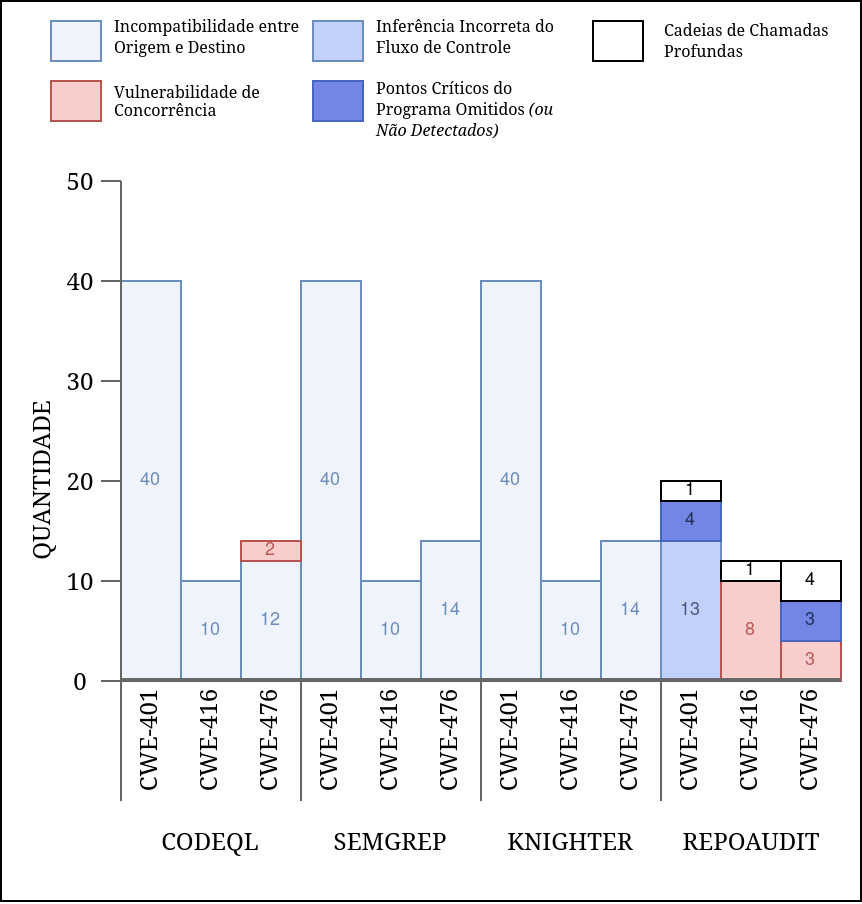
\includegraphics[width=0.46\textwidth]{Images/LLM-Based-Analise.png} \\
    {\vspace{-0.15cm}\scriptsize Fonte: Adaptado para o português para melhor compreensão \cite{li2026llmbased}}
    \label{fig:llmbased}
  \end{figure}
\end{frame}

\begin{frame}{LLM-based Vulnerability Detection...}
  \begin{itemize}
    \item \textbf{\textit{Source-Sink Mismatch}}, definições não correspondem às APIs reais (como \texttt{malloc} e \textt{dev\_alloc\_skb}.
    \item \textbf{\textit{Mis-Inferred Control Flow}}, falha em entender caminhos de execução, como ramificações aninhadas ou definições \texttt{goto}.
    \item \textbf{\textit{Concurrency Vulnerability}}, falha em acompanhar \textit{threads}.
    \item \textbf{\textit{Deep Chains}}, vulnerabilidades que exigem a análise de um contexto profundo de chamadas de funções.
    \item \textbf{\textit{Missed Critical Program Points}}, falha de inferência da LLM ao pular declarações cruciais no meio do código.
  \end{itemize}
\end{frame}

\renewcommand{\minhaspaginas}{\small 43 - 44}
\begin{frame}{Trabalhos relacionados}
  \setbeamerfont{caption}{size=\scriptsize}
  \vspace{-0.88cm} \begin{figure}[h]
    \centering
    \caption{Comparação técnica entre os trabalhos relacionados.}
    \vspace{-0.15cm}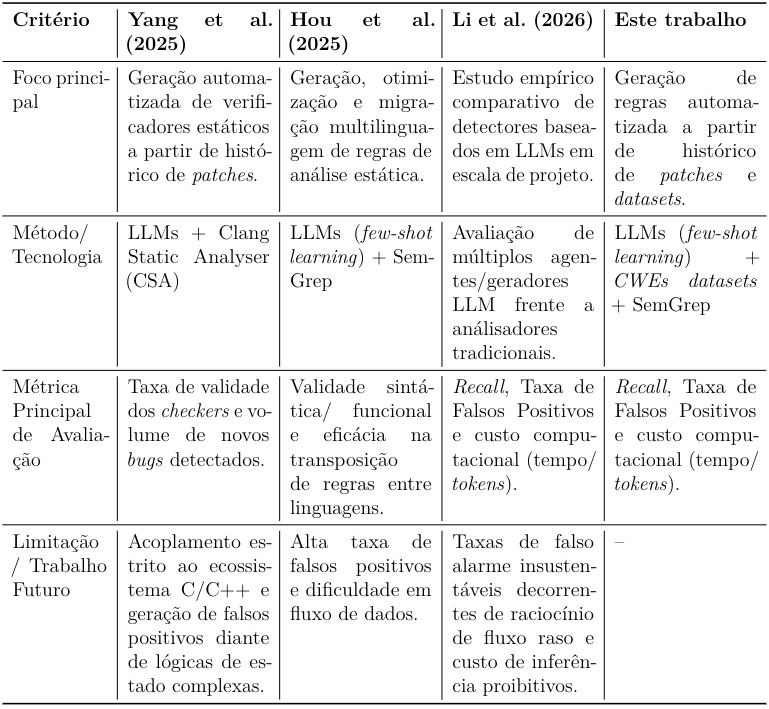
\includegraphics[width=0.54\textwidth]{Images/Table.png} \\
    {\vspace{-0.25cm}\scriptsize Fonte: Elaborado pelo autor (2026)}
    \label{fig:table}
  \end{figure}
\end{frame}

% ---------------------------------------------------------------
\section{Desenvolvimento}
% ---------------------------------------------------------------

\renewcommand{\minhaspaginas}{\small 45}
\begin{frame}{Solução Proposta}
  \begin{itemize}
    \item \textbf{Método utilizado}: 
      \textit{Design Science Research} (DSR), focado na resolução de problemas.
    \item Artefato projetado para otimização da análise estática em projetos de larga escala, realizando uma solução computacional avaliável.
    \item \textbf{Proposta}:
      Extensão Geradora de Regras baseado em LLMs direcionada a Projetos de Larga Escala para a ferramenta de análise estática, SemGrep.
    \item \textbf{Estruturado em quatro fases}:
      \begin{enumerate}
        \item Construção de \textit{dataset};
        \item \textit{Pipeline} de geração de regras;
        \item Avaliação de resultados;
        \item Aplicação no mundo real.
      \end{enumerate}
  \end{itemize}
\end{frame}

\renewcommand{\minhaspaginas}{\small 45 - 46}
\begin{frame}{Arquitetura do trabalho}
  \begin{itemize}
    \item \textbf{Dois módulos independentes}:
      \begin{enumerate}
        \item \textbf{Módulo de \textit{Dataset}}, utilizando o repositório de códigos de \citeonline{nistsard112juliet} e históricos de \textit{commits} de projetos \textit{open-source} ativos;
        \item \textbf{Camada do \textit{Pipeline} (Agentes LLM)}:
          \begin{itemize}
            \item Análise e Abstração (\#1);
            \item Síntese de Sintaxe (\#2);
            \item Assistência e Validação (\#3);
            \item Otimização Contínua e Consolidação de Regras (\#4).
          \end{itemize}
      \end{enumerate}
    \item \textbf{Métricas de avaliação}:
      \begin{itemize}
        \item \textit{Precision}, \textit{Recall} e F1-Score;
        \item Validação Gramática;
        \item Validação Funcional;
        \item Validação em mundo real;
        \item Custo.
      \end{itemize}
  \end{itemize}
\end{frame}

\begin{frame}{Arquitetura do trabalho}
  \vspace{-0.85cm} \begin{figure}[h]
    \centering
    \caption{\textit{Pipeline} para o gerador de regras.}
    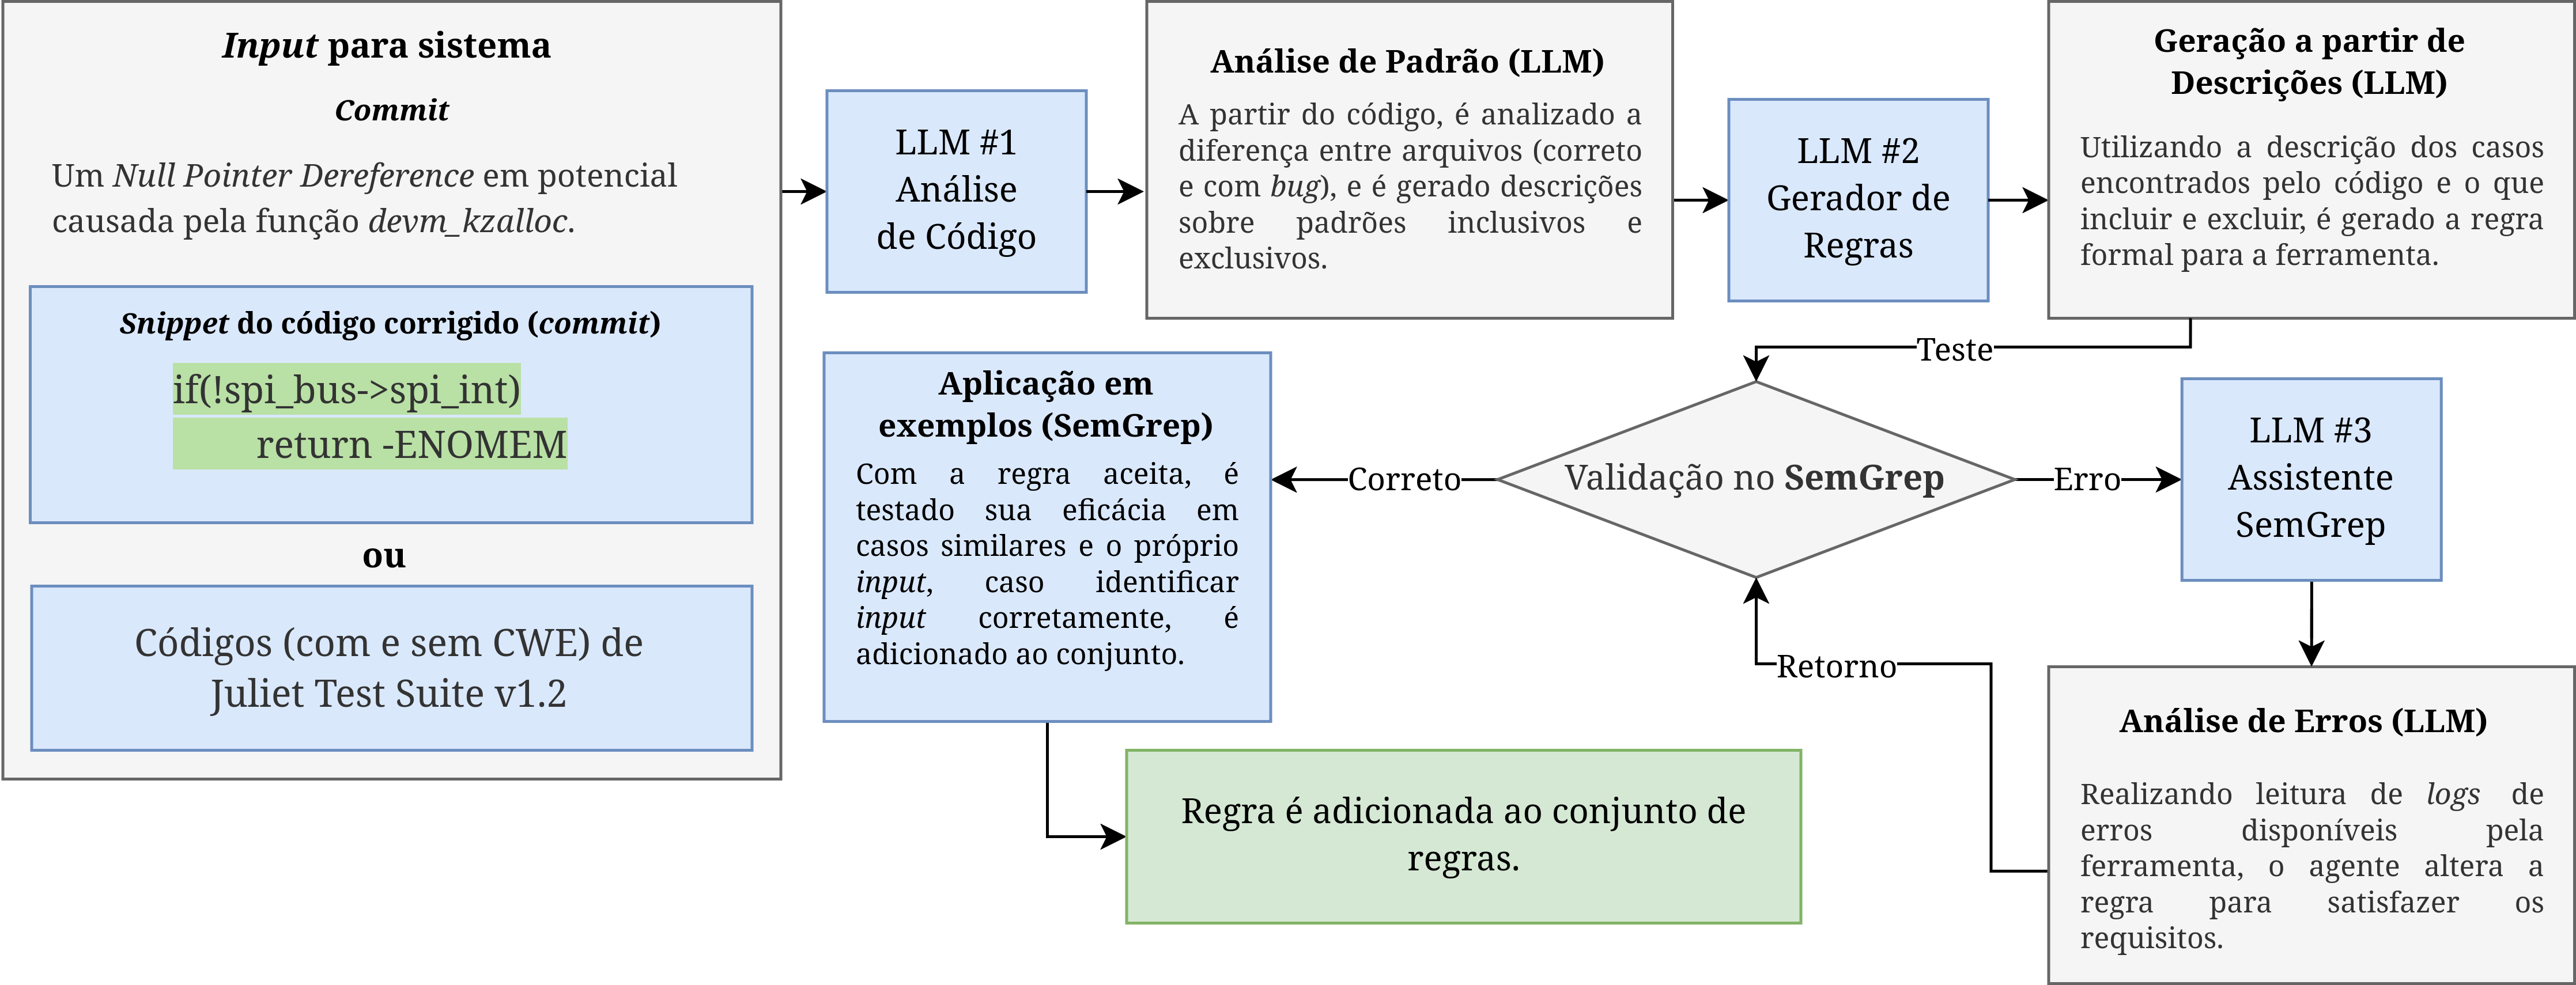
\includegraphics[width=1\textwidth]{Images/Pipeline.png} \\
    {\small Fonte: Elaborado pelo autor (2026)}
    \label{fig:pipeline}
  \end{figure}
\end{frame}

\begin{frame}{Arquitetura do trabalho}
  \vspace{-0.85cm} \begin{figure}[h]
    \centering
    \caption{Pós-processamento para otimizar regras e abranger \textit{corner-cases}.}
    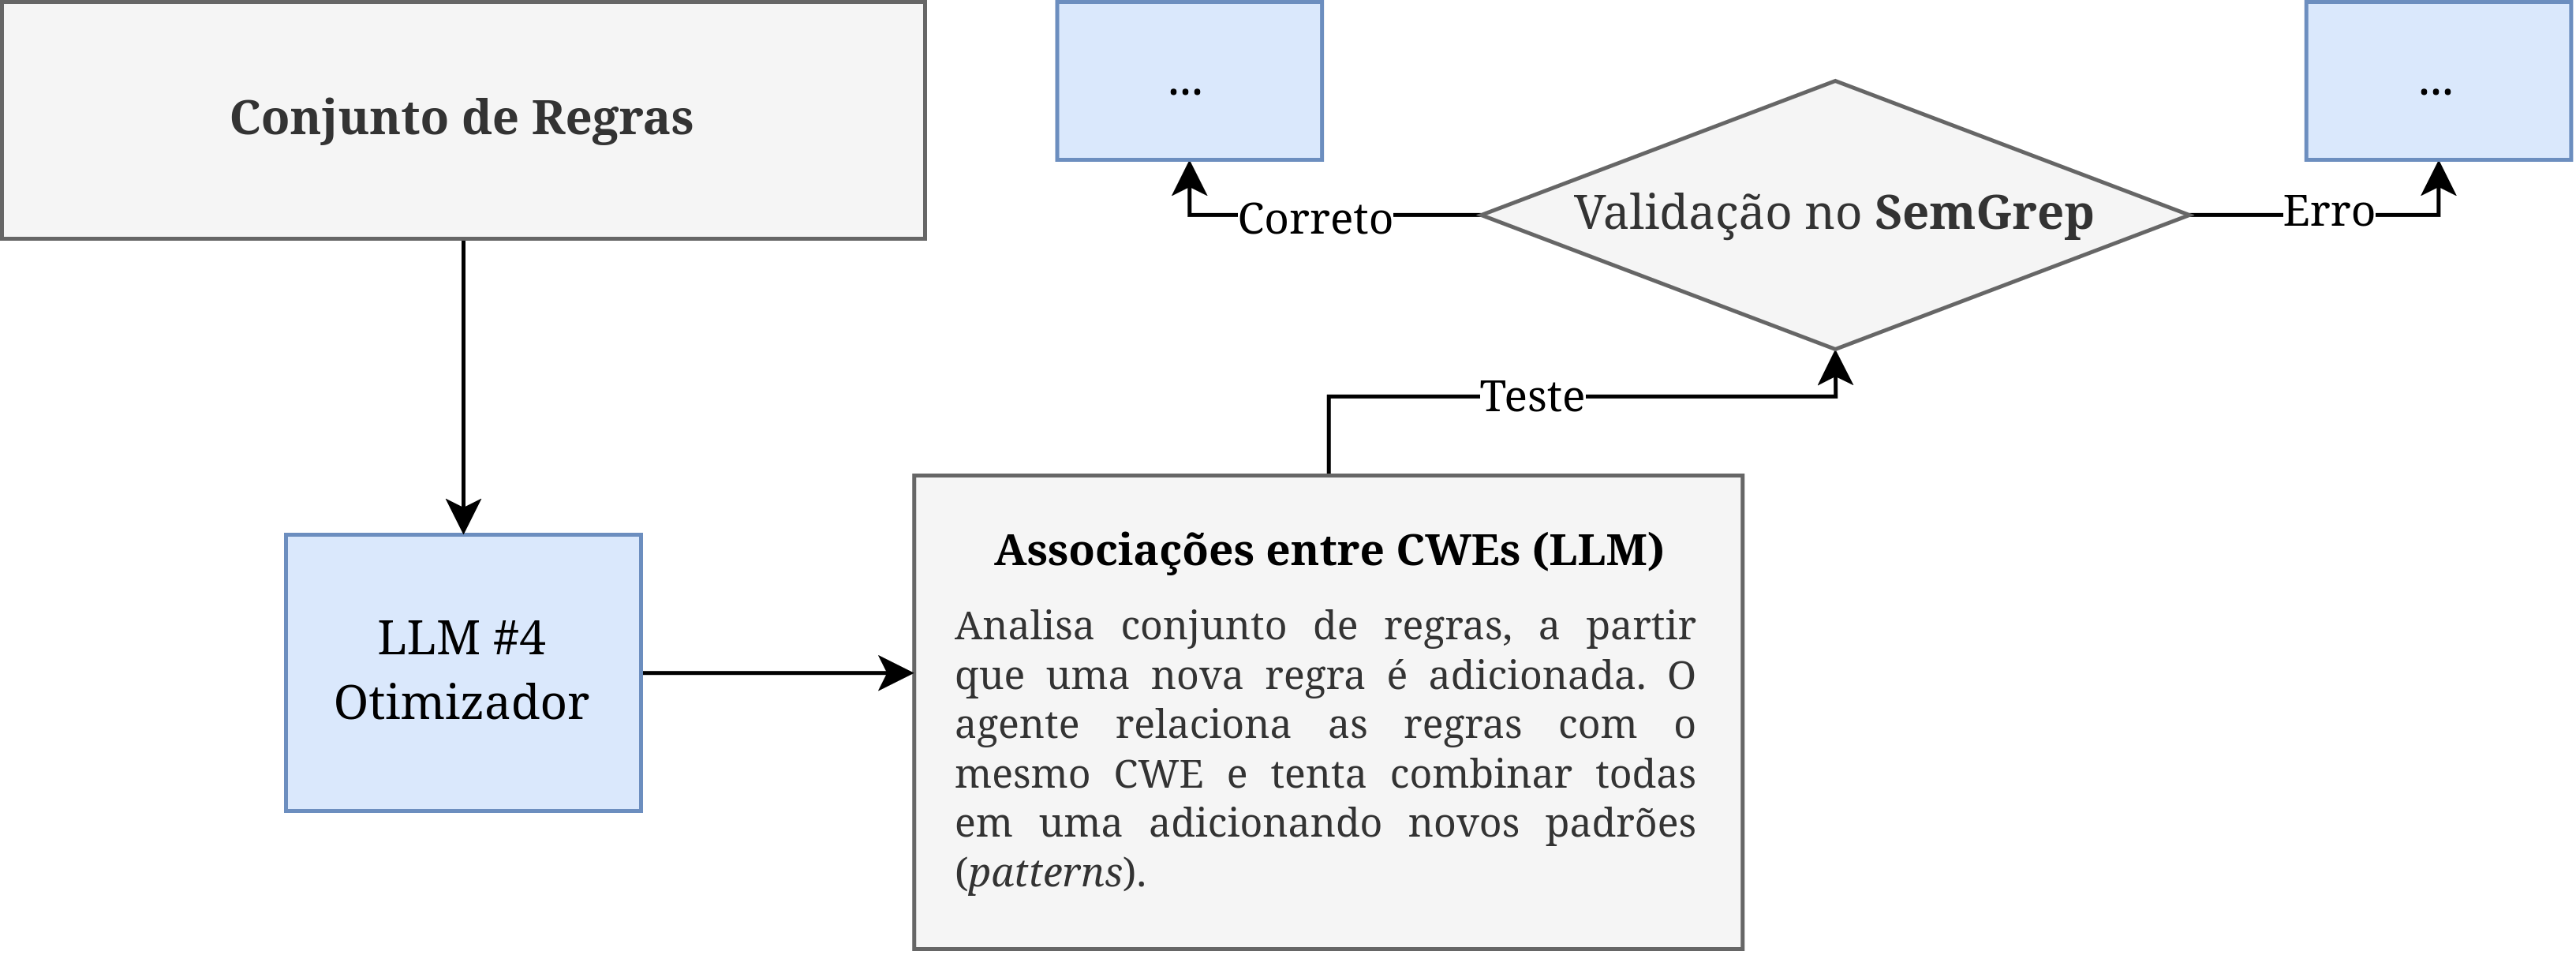
\includegraphics[width=1\textwidth]{Images/QuartoAgente.png} \\
    {\small Fonte: Elaborado pelo autor (2026)}
    \label{fig:quarto}
  \end{figure}
\end{frame}

\renewcommand{\minhaspaginas}{\small 48}
\begin{frame}{Cronograma (TCC2)}
\setbeamerfont{caption}{size=\scriptsize}
  \vspace{-0.88cm} \begin{figure}[h]
    \centering
    \caption{Cronograma de atividades - Diagrama de Gantt.}
    \vspace{-0.2cm}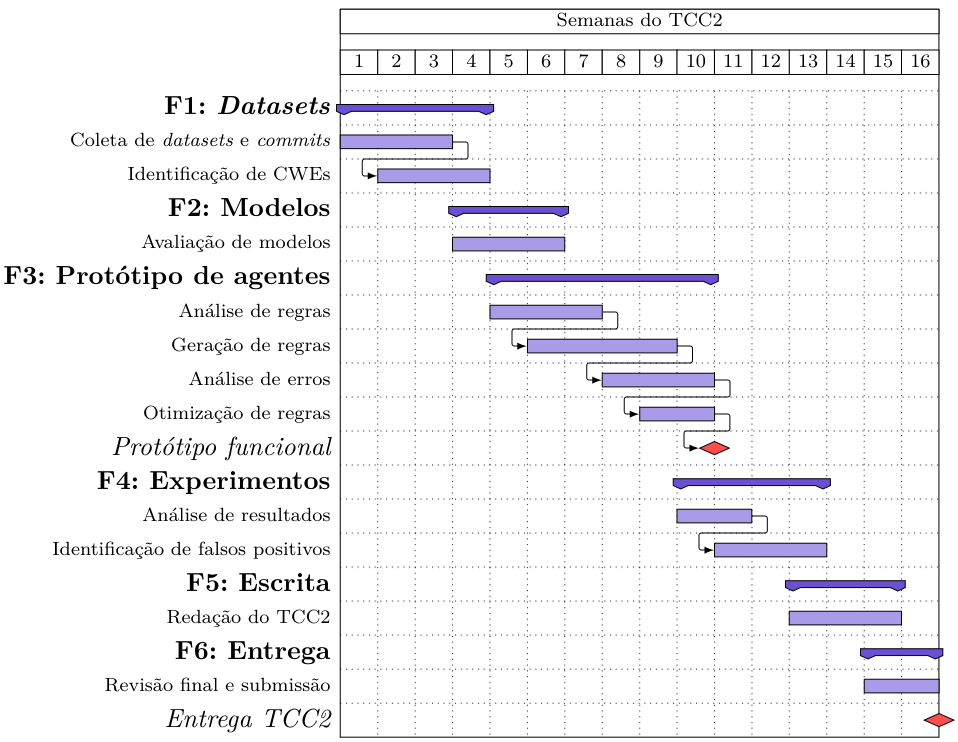
\includegraphics[width=0.65\textwidth]{Images/Cronograma.png} \\
    {\vspace{-0.25cm}\scriptsize Fonte: Elaborado pelo autor (2026)}
    \label{fig:cronograma}
  \end{figure}

\end{frame}

\renewcommand{\minhaspaginas}{\small}
\begin{frame}[plain]
  \centering
  \vspace{1cm}\logosenacgrande \\
  \vspace{0.8cm}{\Large\bfseries\color{senacblue}Obrigado!\par} 
  \vspace{0.3cm}{\normalsize Perguntas?\par}
  \vspace{0.6cm}{\footnotesize Caio Xavier da Silva \\ caioxaviercxs@gmail.com}
\end{frame}

% ---------------------------------------------------------------
% APÊNDICE (slides de apoio / backup para perguntas da banca)
% ---------------------------------------------------------------
\appendix
\begin{frame}[allowframebreaks]{Referências}
  % Escolha o estilo do seu curso (ex: sbc, plain, abntex2-alf)
  \bibliographystyle{abntex2-alf} 
  \bibliography{bibliografia}
\end{frame}

\end{document}
